
\clearpage

\section{$\HT$ tail dedicated control regions}\label{app:htx_httail}

A study has been performed to identify a set of cuts that could deplete the signal
contribution at high $\HT$ but still leave enough background contribution 
to check the Standard Model bagrounds modeling for the signal region blinded
in the control regions previously described. 
The signal veto cut studied is an upper cut on the number 
of jets above a given $\pt$ threshold, higher than the usual $\pt>25\gev$. 
For different thresholds
the $S/B$ ratio was estimated as a function of $\HT$ for 
each of the three analysis channels separately (\chii, \chiii\ and \chiv) 
and for two extreme signal scenarios (vector-like quark doublet and chiral 
fourth generation quark with $BR(\T \to Wb)=1$, both with $m_{\T}=600\gev$),
characterized by very different topologies and therefore differently affected by any additional
signal veto cuts applied, and a $\HT$ region with $S/B\leq 10\%$ per bin
and sufficient statistical populetion was identified.
It was found that the distribution of number of 
jets with $\pt>60\gev$ offers reasonable discrimination 
between the $t\bar{t}$ background and the two 
signal scenarios.% as illustrated in in Fig.~\ref{fig:blinding_on_Njets_6jetin2btagex}.
For a requirement $\leq 2$ jets with $\pt>60\gev$ 
about 35\% of the $t\bar{t}$ background remains while the signal is suppressed
by a factor $\sim 30$. 
Admittedly, this cut selects a subset of background events where the high $\HT$ region will be populated
by events with at most two hard jets and possibly large lepton $\pt$ and $\met$ and high multiplicity of lower-$\pt$ jets. 
Nevertheless, it is useful to be able to probe the high $\HT$ tail for at least a subset of the background
%The next step is to determine up to which value of $\HT$ can the distribution be scrutinized without being too much contaminated
%by a potential signal. Figure~\ref{fig:blinding_on_Njets_HT} shows the expected $S/B$ as a function of $\HT$ for events selected with the veto
%requirement discussed above ($\leq 2$ jets with $\pt>60\gev$) in the three channels considered in the search.  
It was then found that in the \chii\ and \chiii\ channels the $\HT$ distribution 
could be examined  up to $1.2\tev$ with an expected $S/B\leq 10\%$ per bin for 
either of the two signal scenarios considered. In the case of the \chiv\ channel, 
it was not possible to go significantly
above the original blinding cut of $700\gev$. 
Being able to go up to $\HT\sim 1.2\tev$ probes the kinematic region where a $\T$
signal with $m_{\T}=600\gev$ would peak and therefore constitues a useful control region for the background.
Therefore, the control region to examine the high $\HT$ tail are defined as: selected events with 2 $b$-tags or  3 $b$-tags, 
$\leq 2$ jets with $\pt>60\gev$, and $\HT<1.2\tev$.  
The comparisons between data and prediction (using scaled $t\bar{t}$ {\sc Alpgen}) 
in this control region, including the expected pre-fit systematic uncertainties, are shown
in Figure~\ref{fig:httailHTAll}.


%
%%%%%%%%%%%%%%
\begin{figure}[htbp]
\begin{center}
\begin{tabular}{ccc}
%
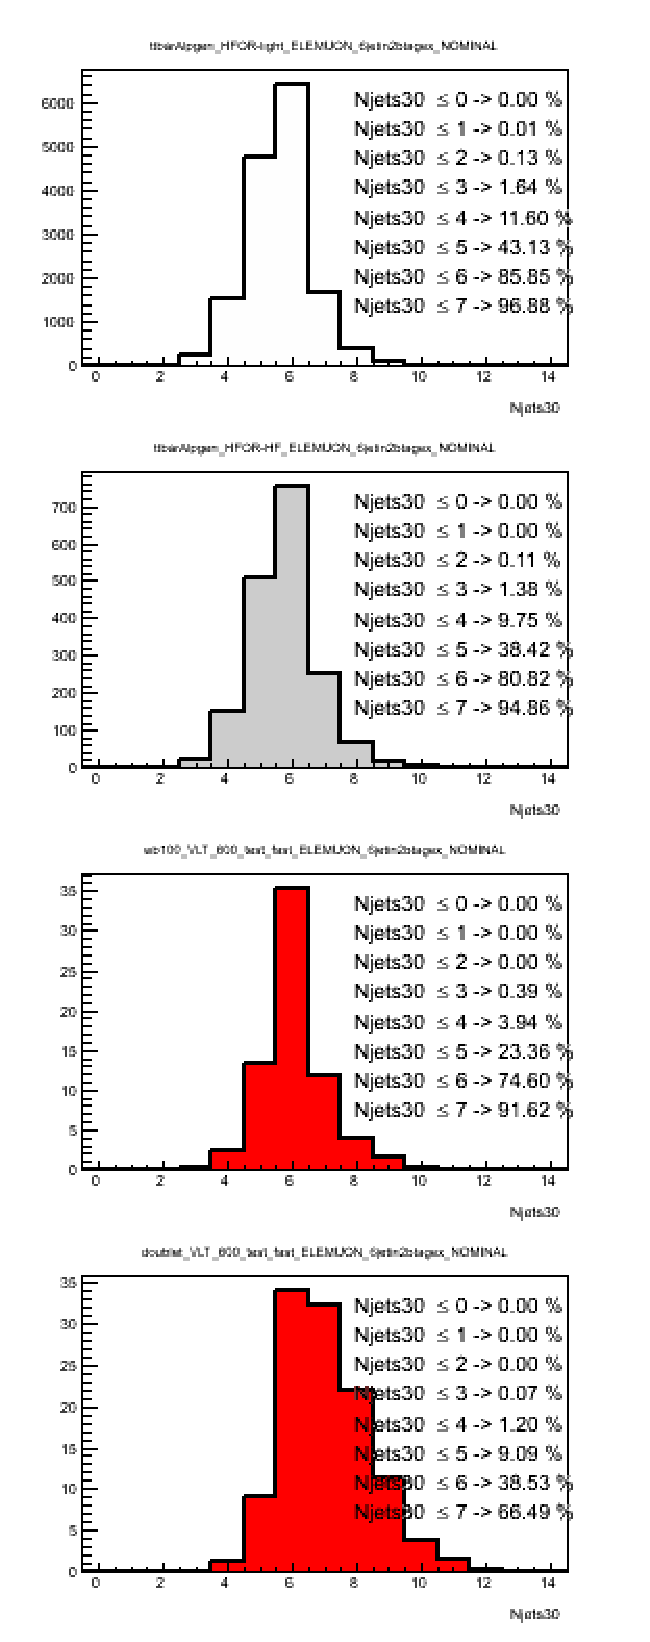
\includegraphics[width=0.33\textwidth]{appendices/figures/htx_httail/blinding_on_Njets30__ELEMUON_6jetin2btagex_NOMINAL.eps} &
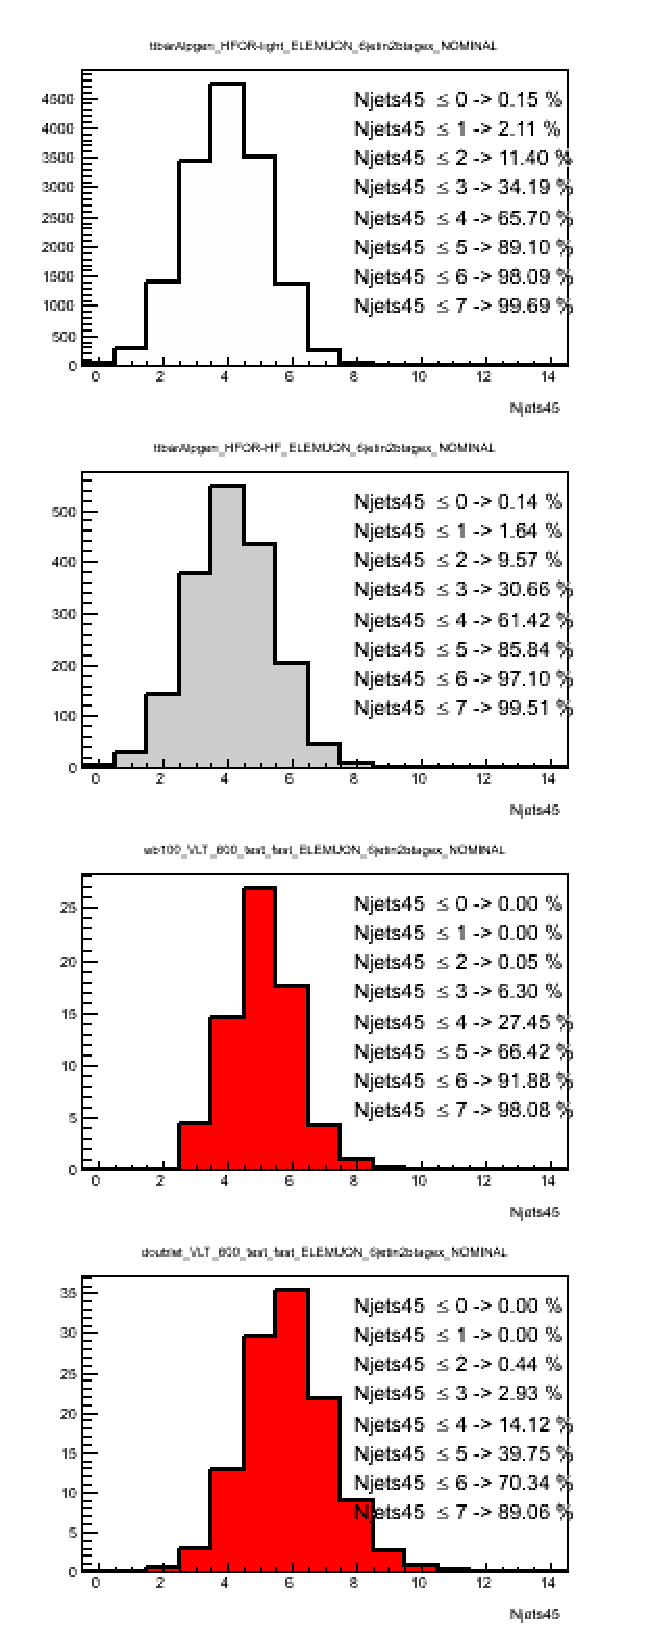
\includegraphics[width=0.33\textwidth]{appendices/figures/htx_httail/blinding_on_Njets45__ELEMUON_6jetin2btagex_NOMINAL.eps} &
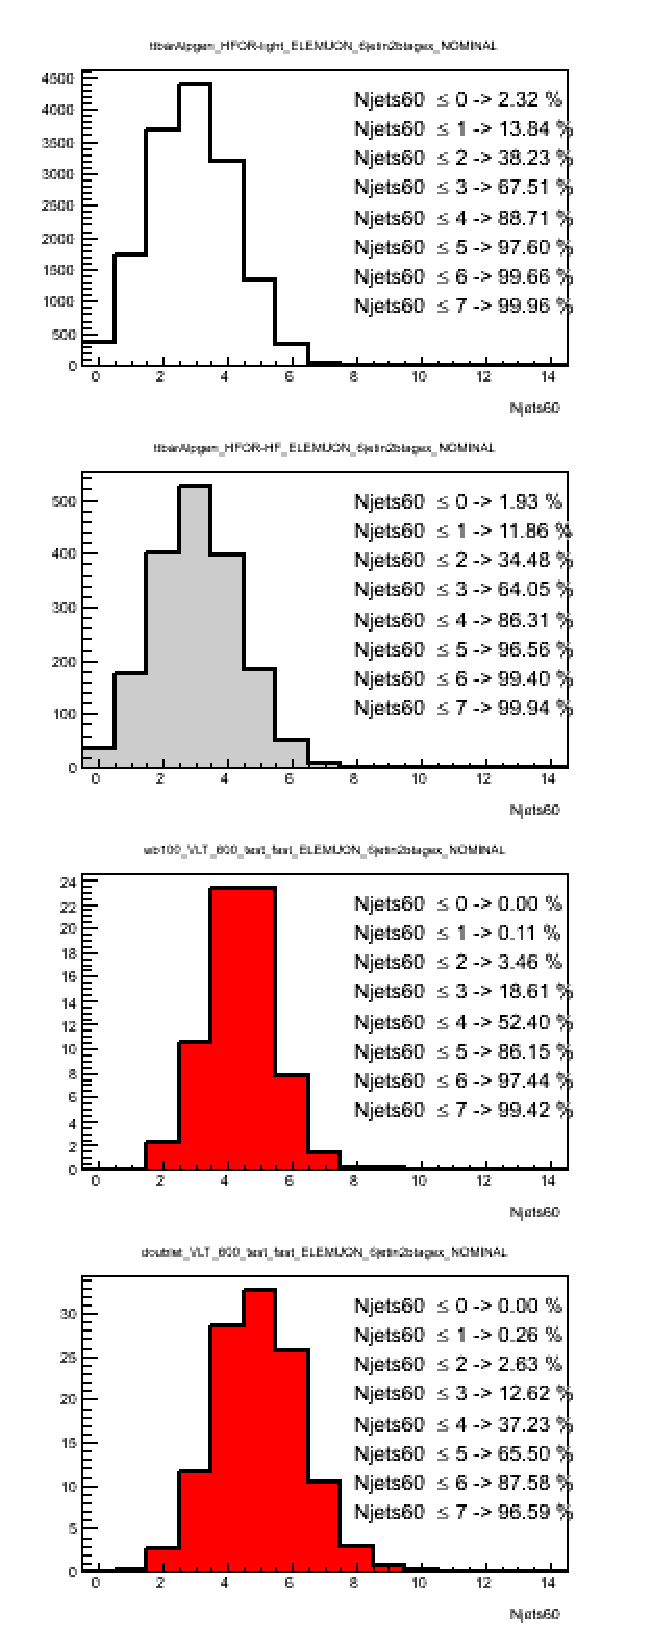
\includegraphics[width=0.33\textwidth]{appendices/figures/htx_httail/blinding_on_Njets60__ELEMUON_6jetin2btagex_NOMINAL.eps} \\
\end{tabular}\caption{\small {Jet multiplicity distribution corresponding to minimum $\pt$ thresholds of (left) $30\gev$, (center) $45\gev$ and (right) $60\gev$ for events in the 2 $b$-tags channel after final selection. From top to bottom the following processes are compared: $t\bar{t}$+light jets, $t\bar{t}$+heavy-flavour jets, chiral 4th generation $\T$ signal ($m_{\T}=600\gev$), vector-like $\T$ doublet ($m_{\T}=600\gev$). }}
\label{fig:blinding_on_Njets_6jetin2btagex}
\end{center}
\end{figure}
%%%%%%%%%%%%%%




%%%%%%%%%%%%%%
\begin{figure}[h!tb]
\begin{center}
\begin{tabular}{ccc}
%
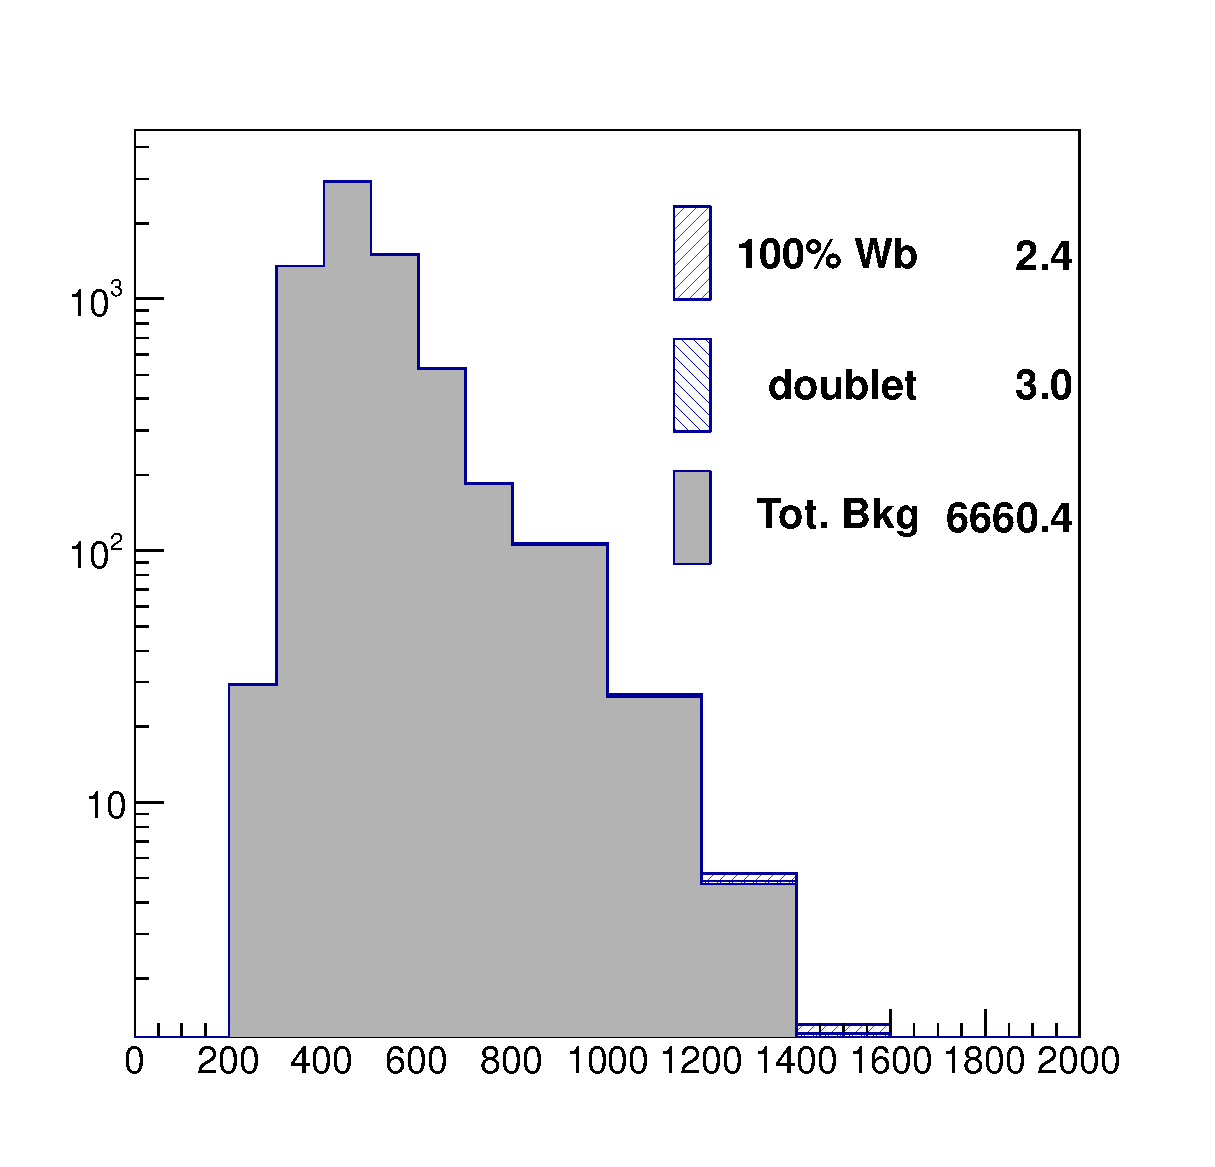
\includegraphics[width=0.3\textwidth]{appendices/figures/htx_httail/var_HTAll_MUON_6jetin2btagex_Njets60lower3} &
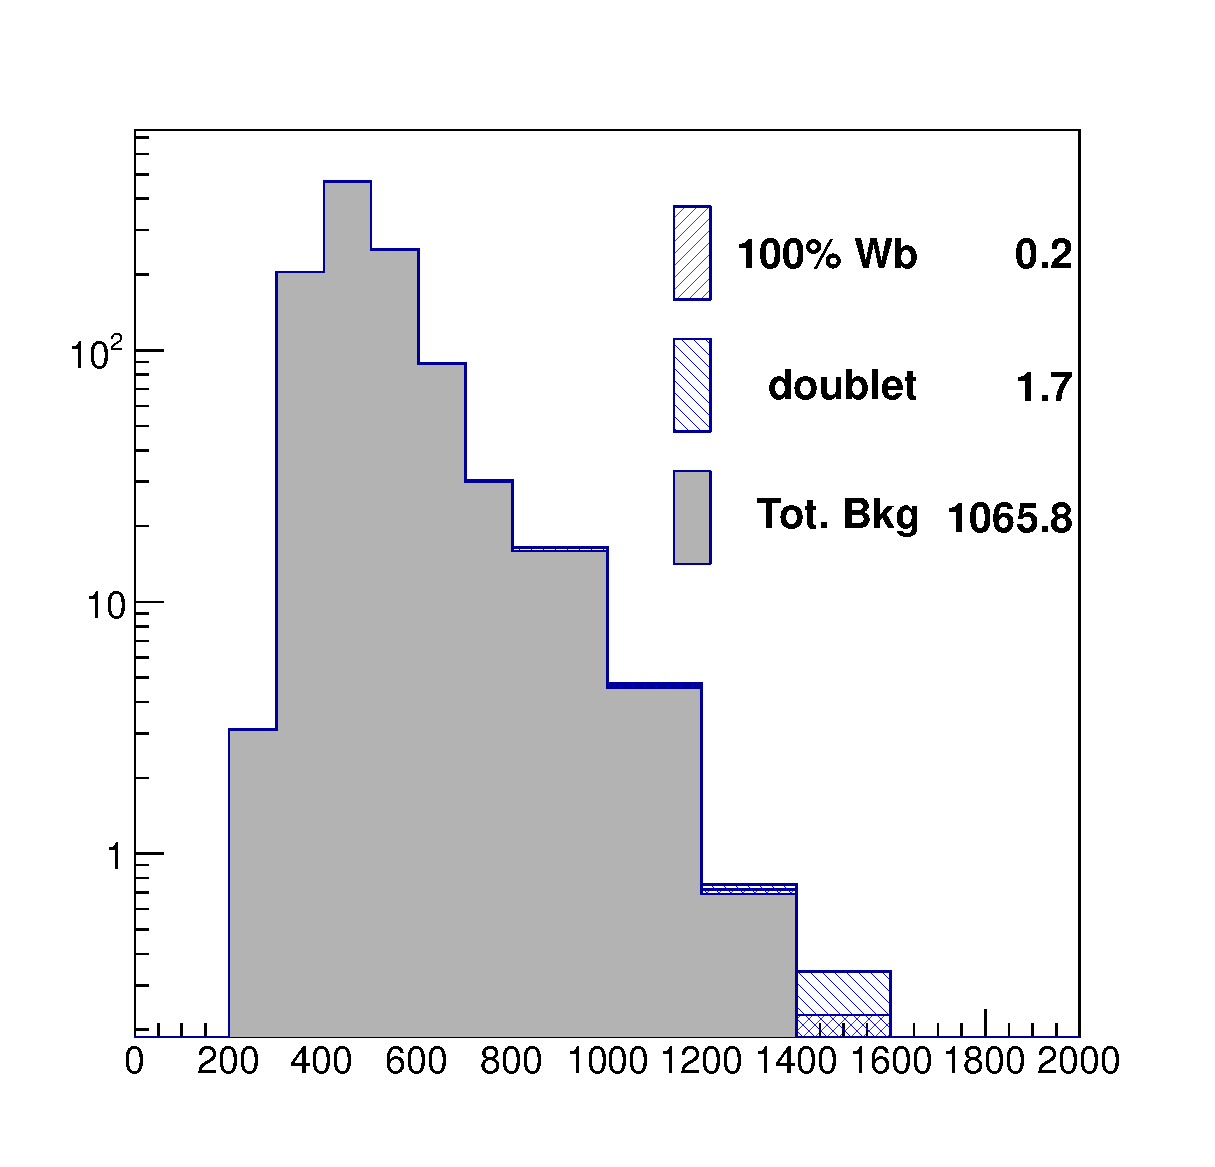
\includegraphics[width=0.3\textwidth]{appendices/figures/htx_httail/var_HTAll_MUON_6jetin3btagex_Njets60lower3} &
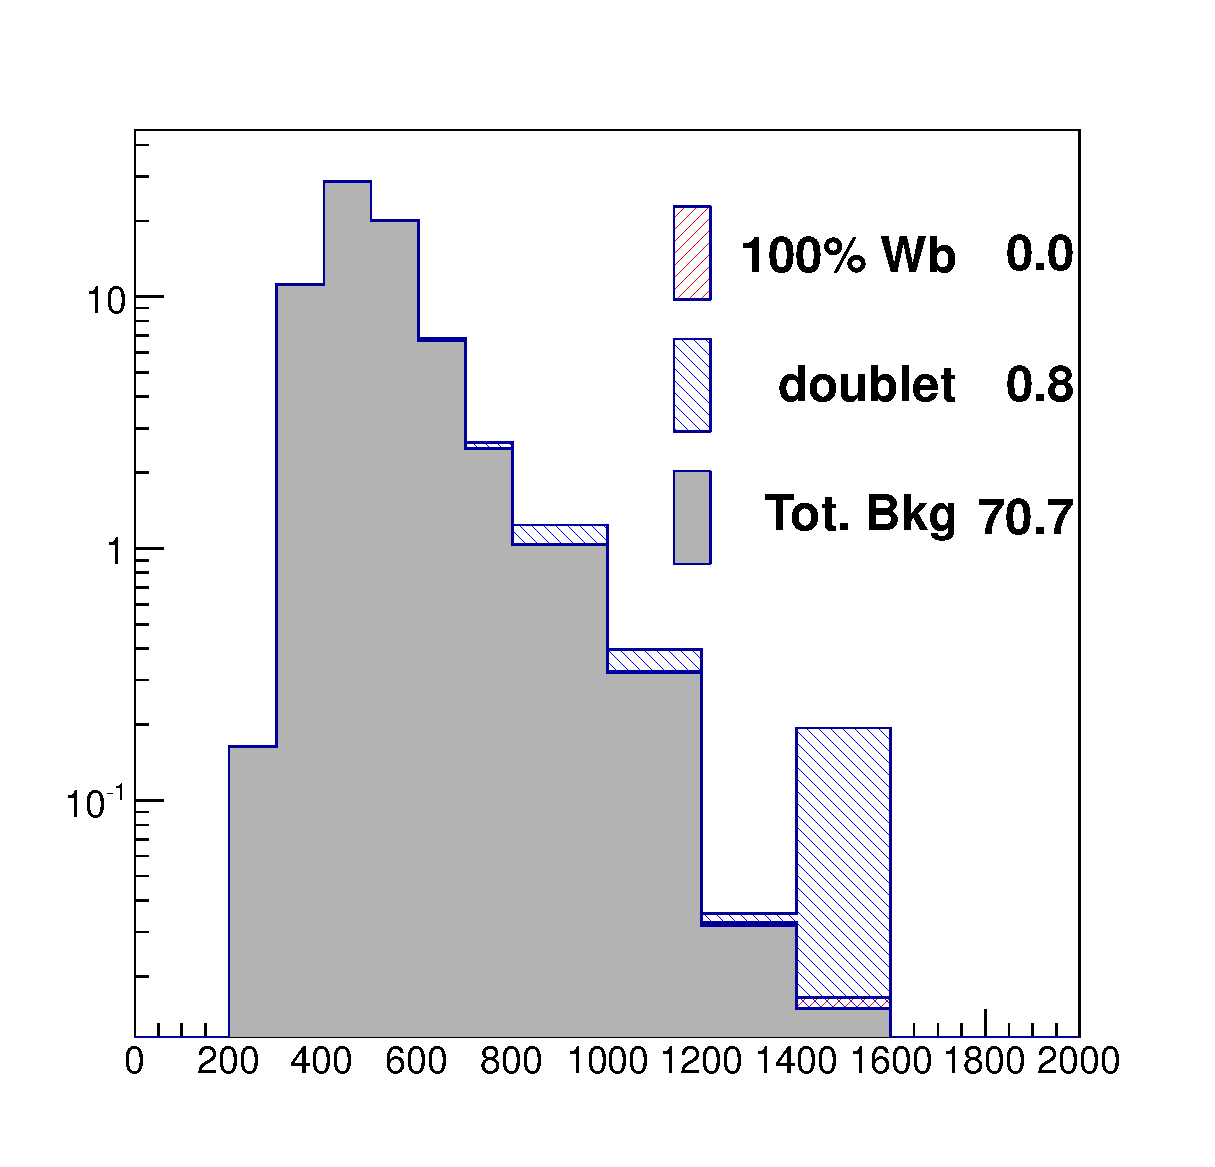
\includegraphics[width=0.3\textwidth]{appendices/figures/htx_httail/var_HTAll_MUON_6jetin4btagin_Njets60lower3} \\
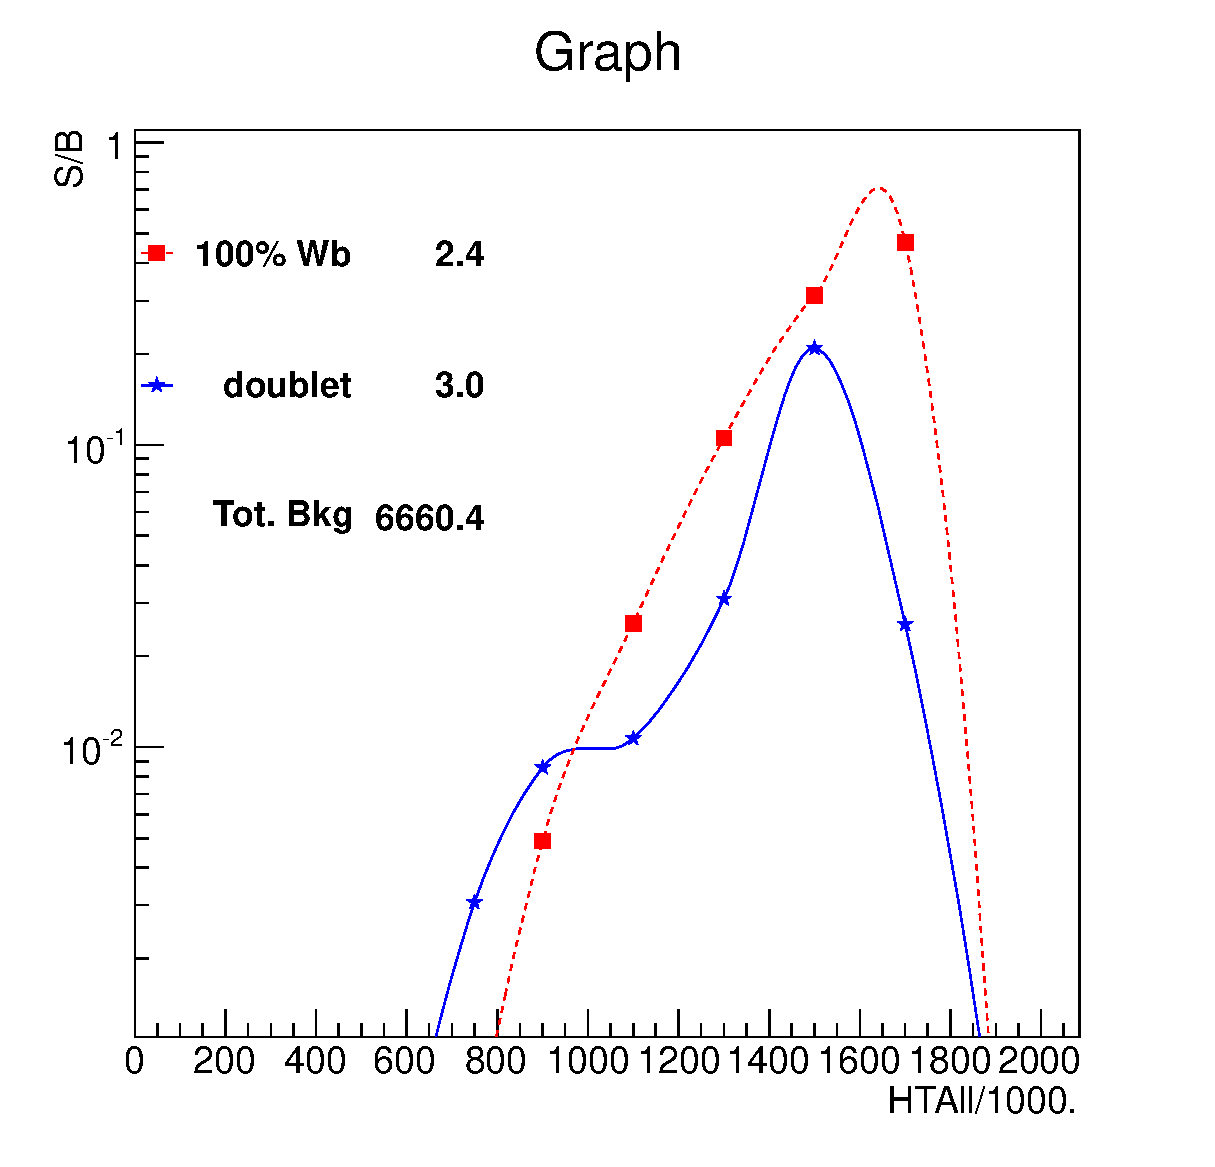
\includegraphics[width=0.3\textwidth]{appendices/figures/htx_httail/sb_HTAll_MUON_6jetin2btagex_Njets60lower3} &
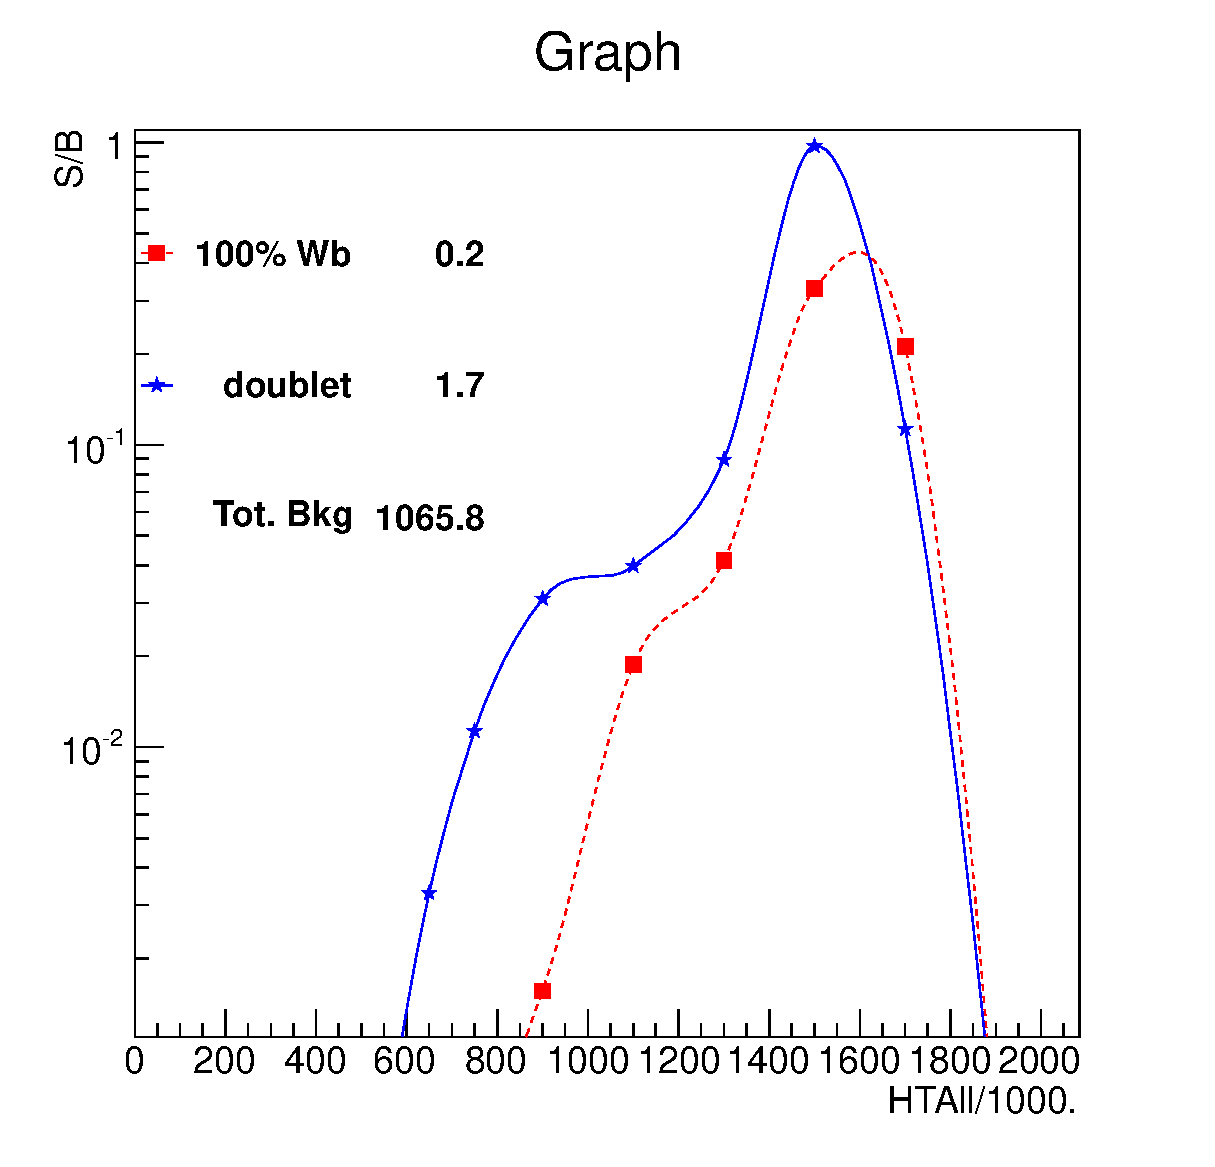
\includegraphics[width=0.3\textwidth]{appendices/figures/htx_httail/sb_HTAll_MUON_6jetin3btagex_Njets60lower3} &
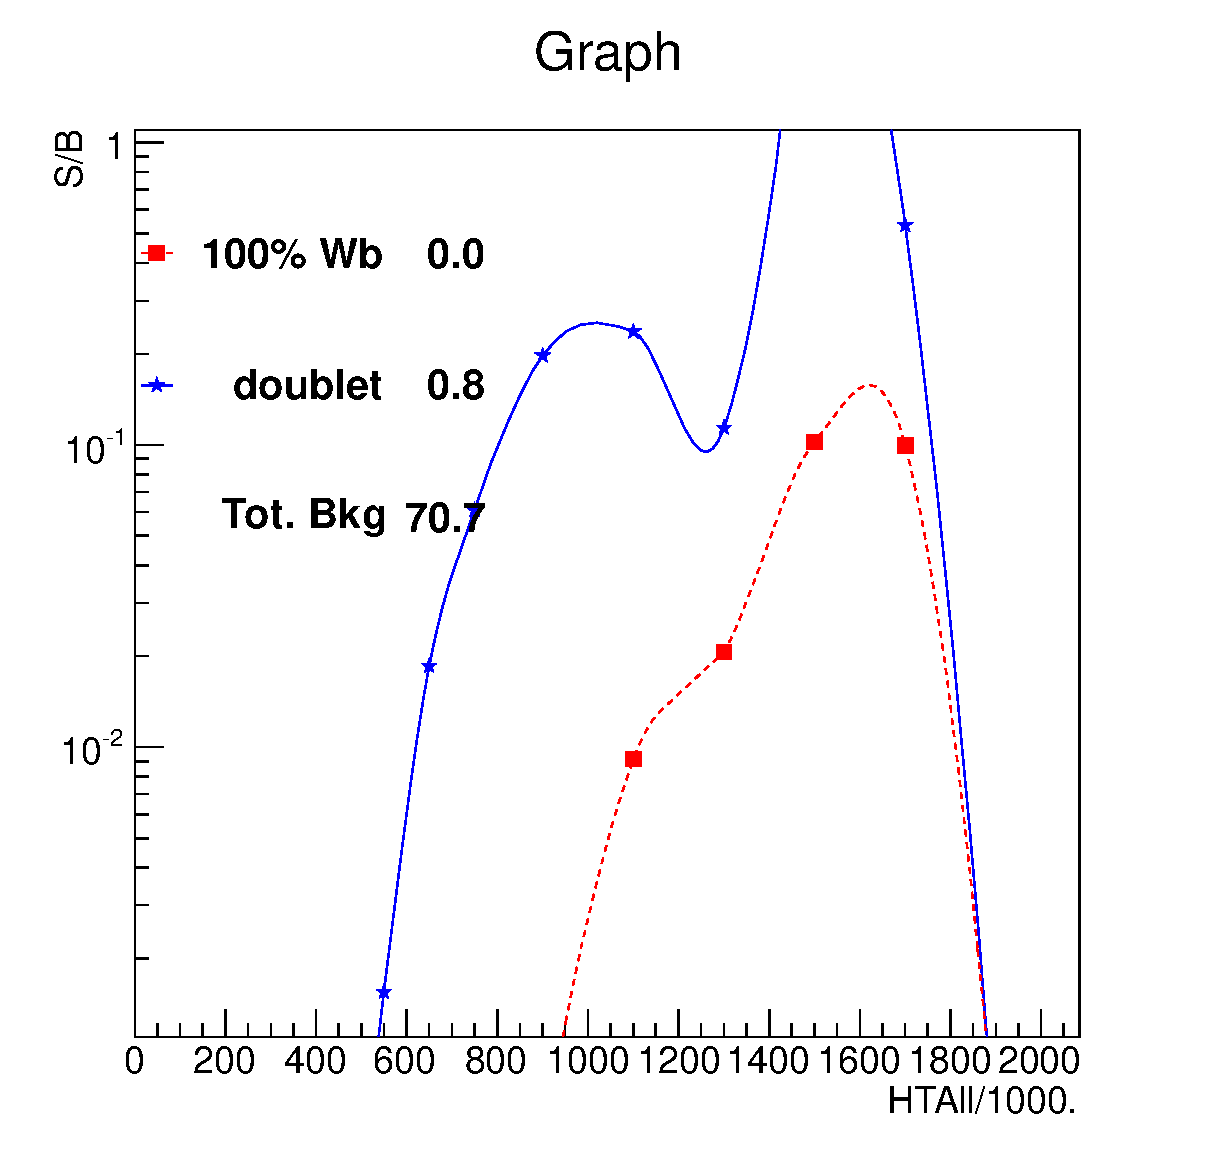
\includegraphics[width=0.3\textwidth]{appendices/figures/htx_httail/sb_HTAll_MUON_6jetin4btagin_Njets60lower3} \\
\end{tabular}\caption{Top: Expected $\HT$ distribution for events after final selection and including the
requirement of $\leq 2$ jets with $\pt>60\gev$, in the (left) 2 $b$-tags, (center) 3 $b$-tags and (right) $\geq 4$ $b$-tags channels.
Shown is the spectrum for total background background as well as the expected signal in the two scenarios considered
(see text for details). Bottom: Expected $S/B$ as a function of $\HT$ after final selection and including the
requirement of $\leq 2$ jets with $\pt>60\gev$, in the (left) 2 $b$-tags, (center) 3 $b$-tags and (right) $\geq 4$ $b$-tags channels.
The two signal scenarios considered are shown.\label{fig:blinding_on_Njets_HT}}
	\subfigure[]{
  	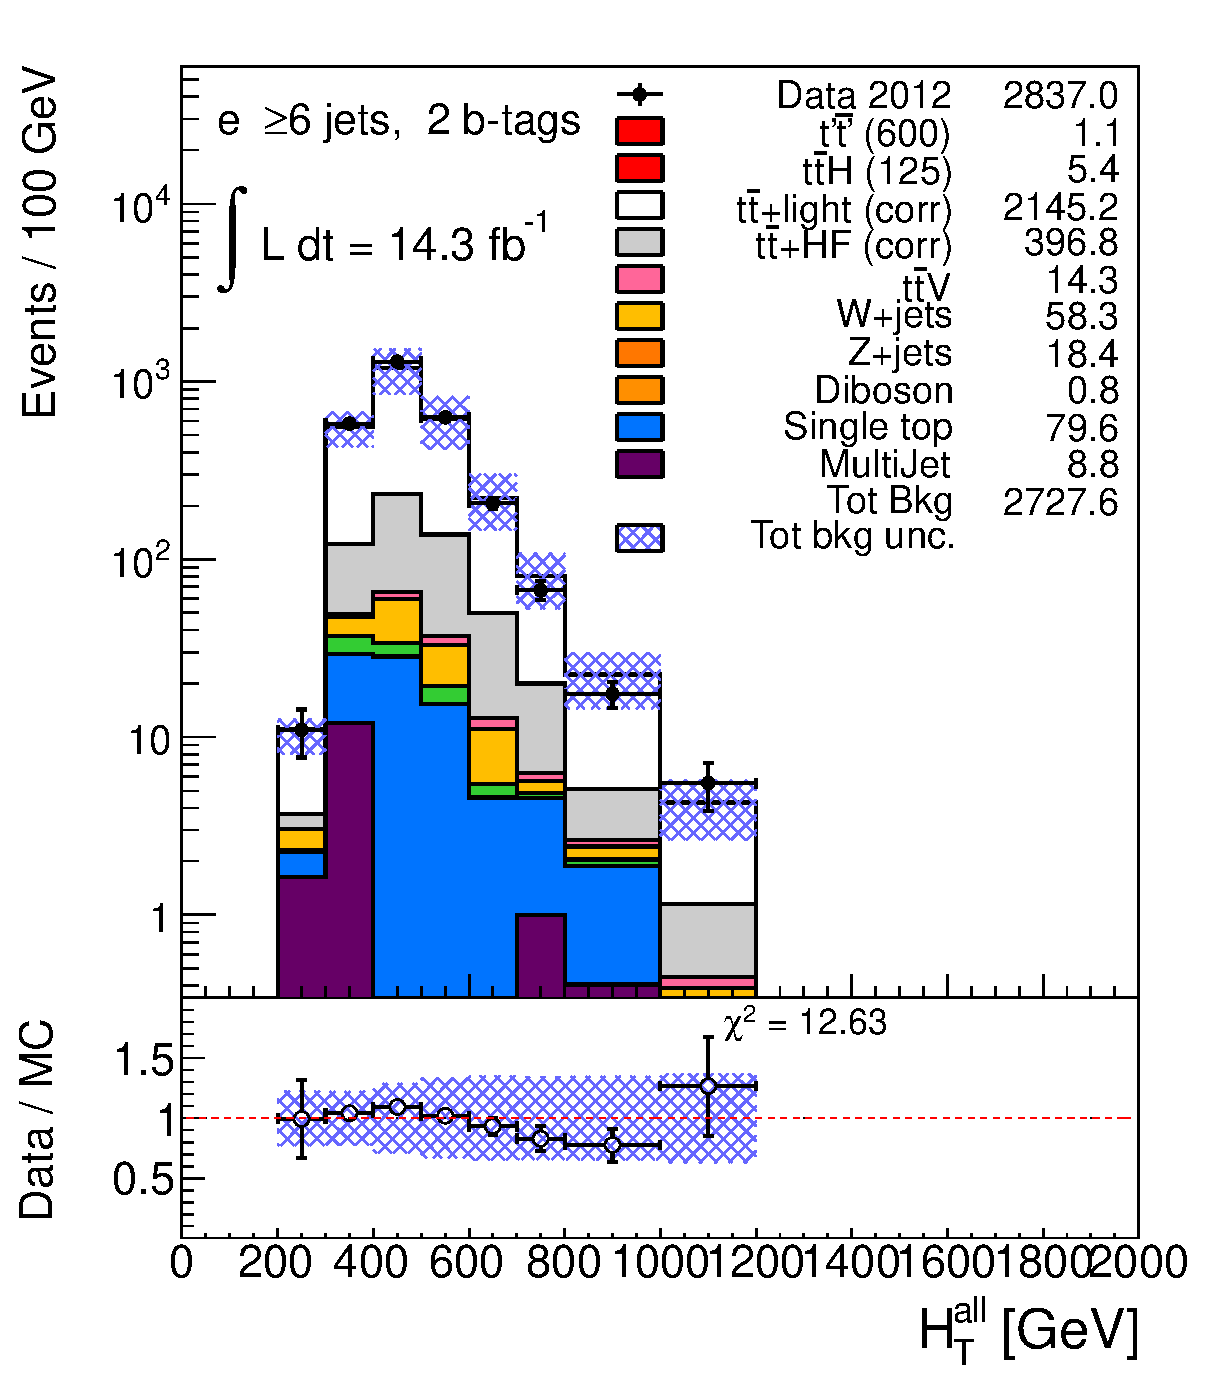
\includegraphics[width=0.3\textwidth]{appendices/figures/htx_httail/HTAll_ELE_6jetin2btagex_NOMINAL_logscale.eps}}
	\subfigure[]{
  	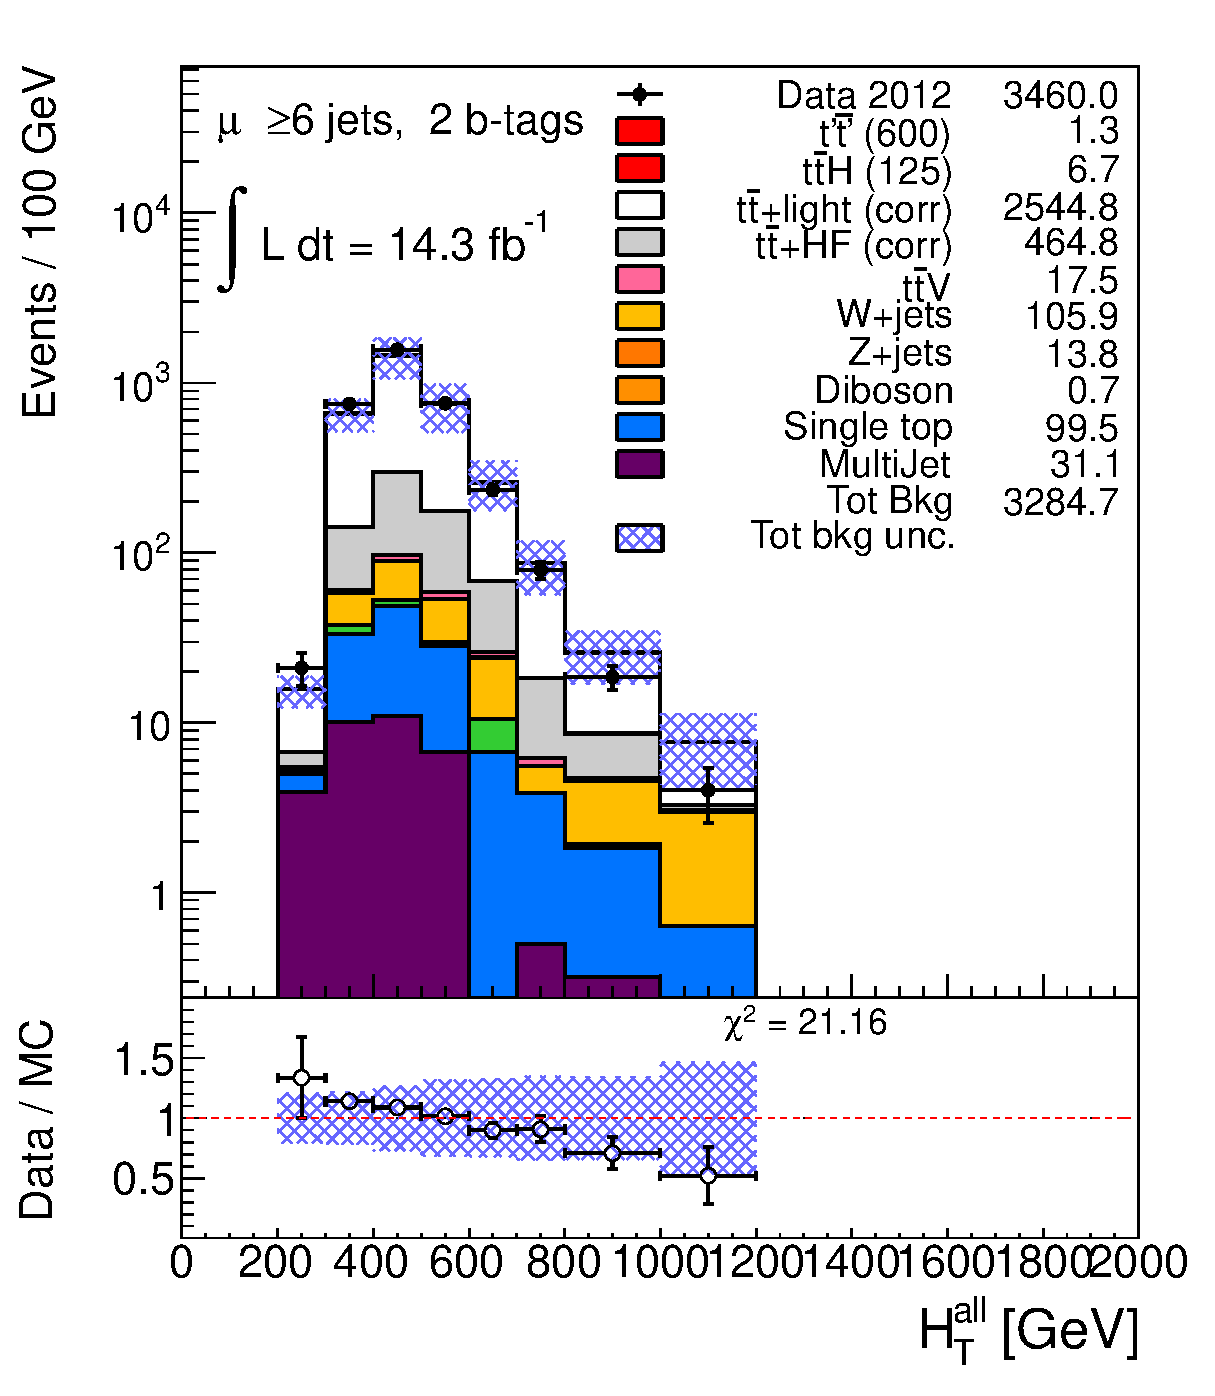
\includegraphics[width=0.3\textwidth]{appendices/figures/htx_httail/HTAll_MUON_6jetin2btagex_NOMINAL_logscale.eps}}
	\subfigure[]{
  	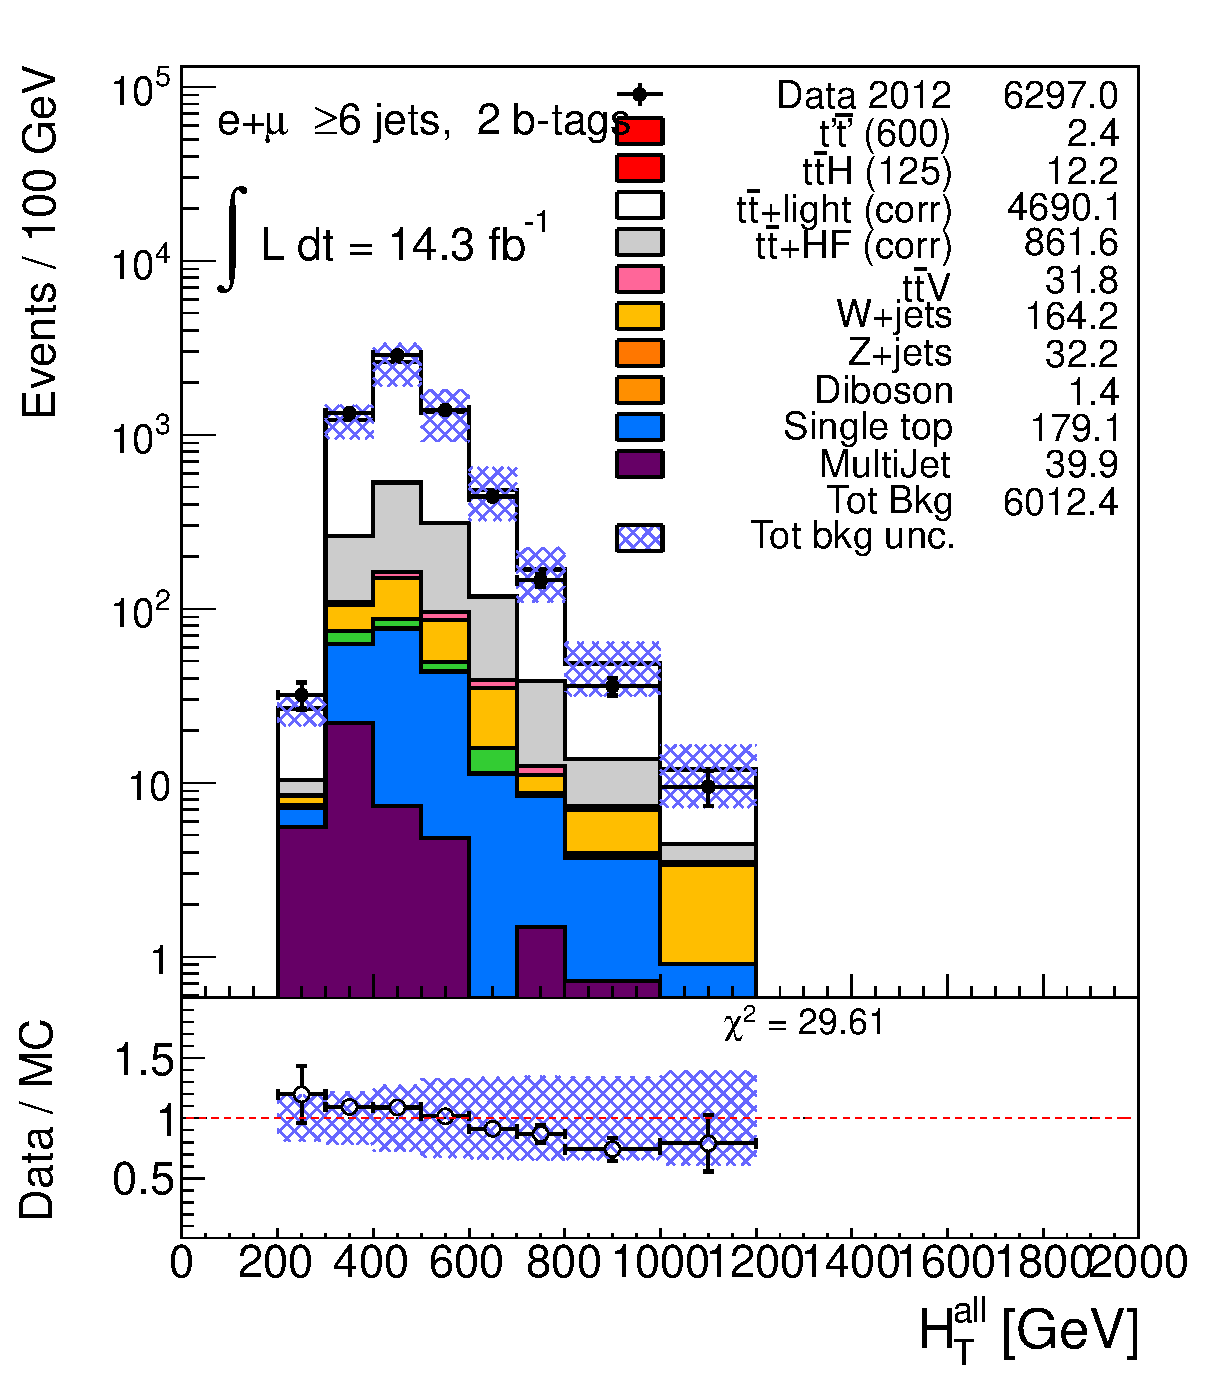
\includegraphics[width=0.3\textwidth]{appendices/figures/htx_httail/HTAll_ELEMUON_6jetin2btagex_NOMINAL_logscale.eps}}
	\subfigure[]{
  	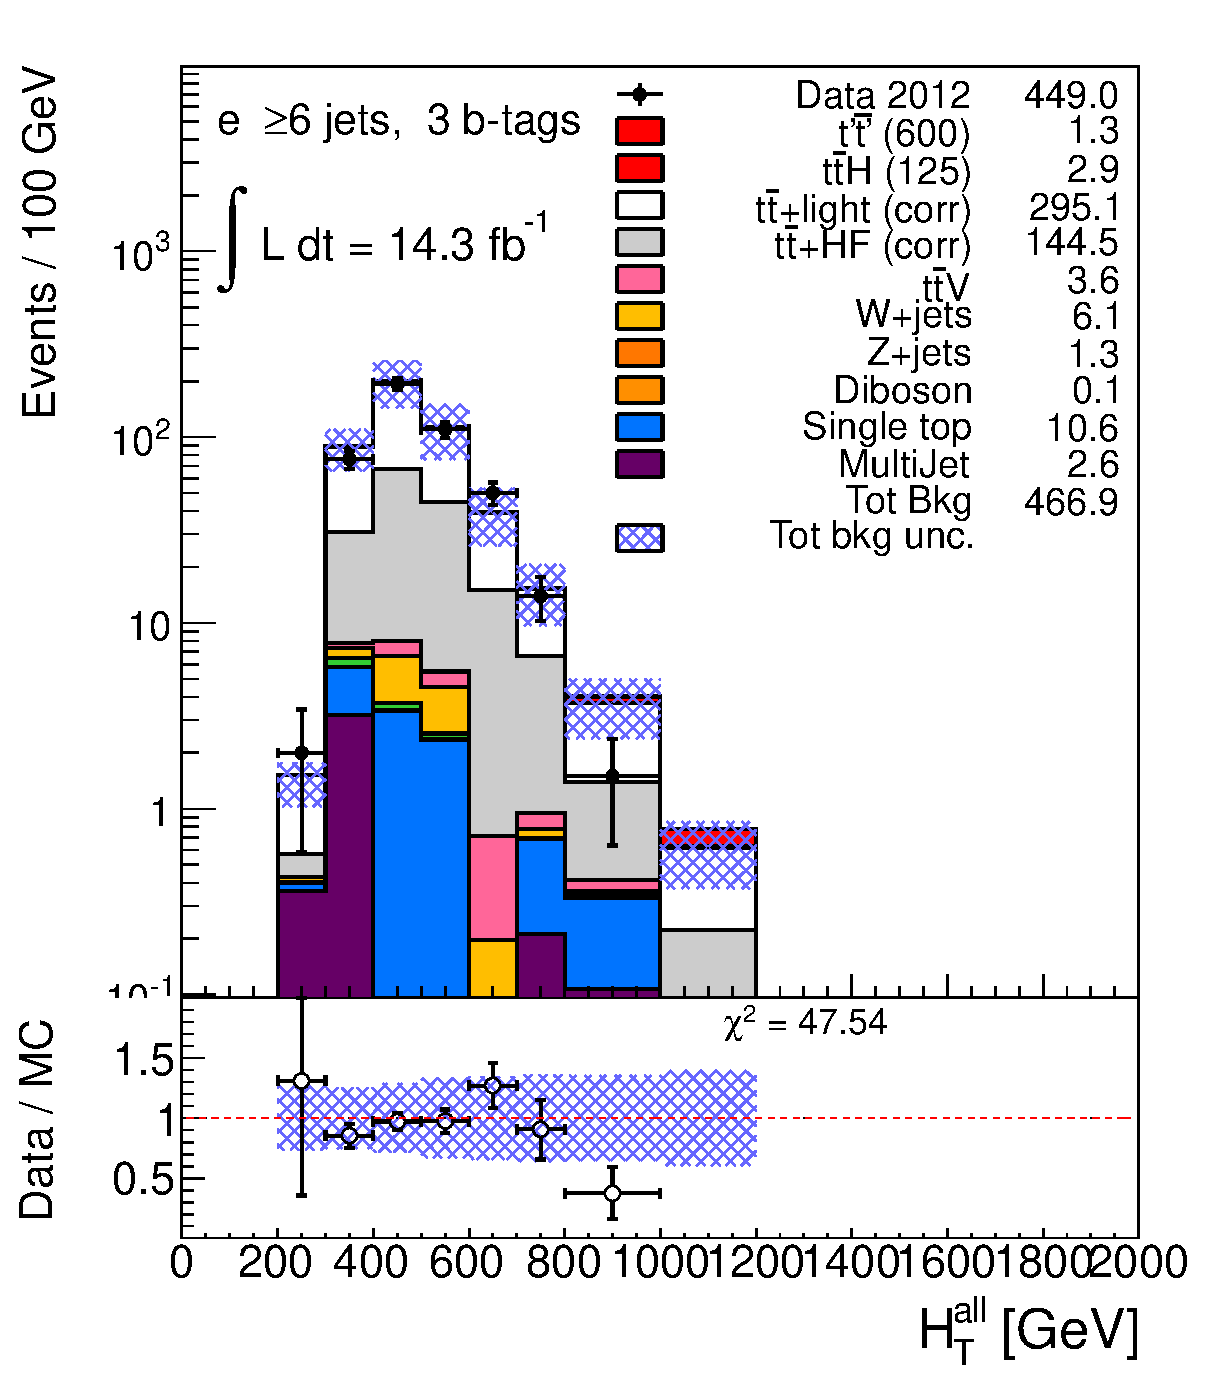
\includegraphics[width=0.3\textwidth]{appendices/figures/htx_httail/HTAll_ELE_6jetin3btagex_NOMINAL_logscale.eps}}
	\subfigure[]{
  	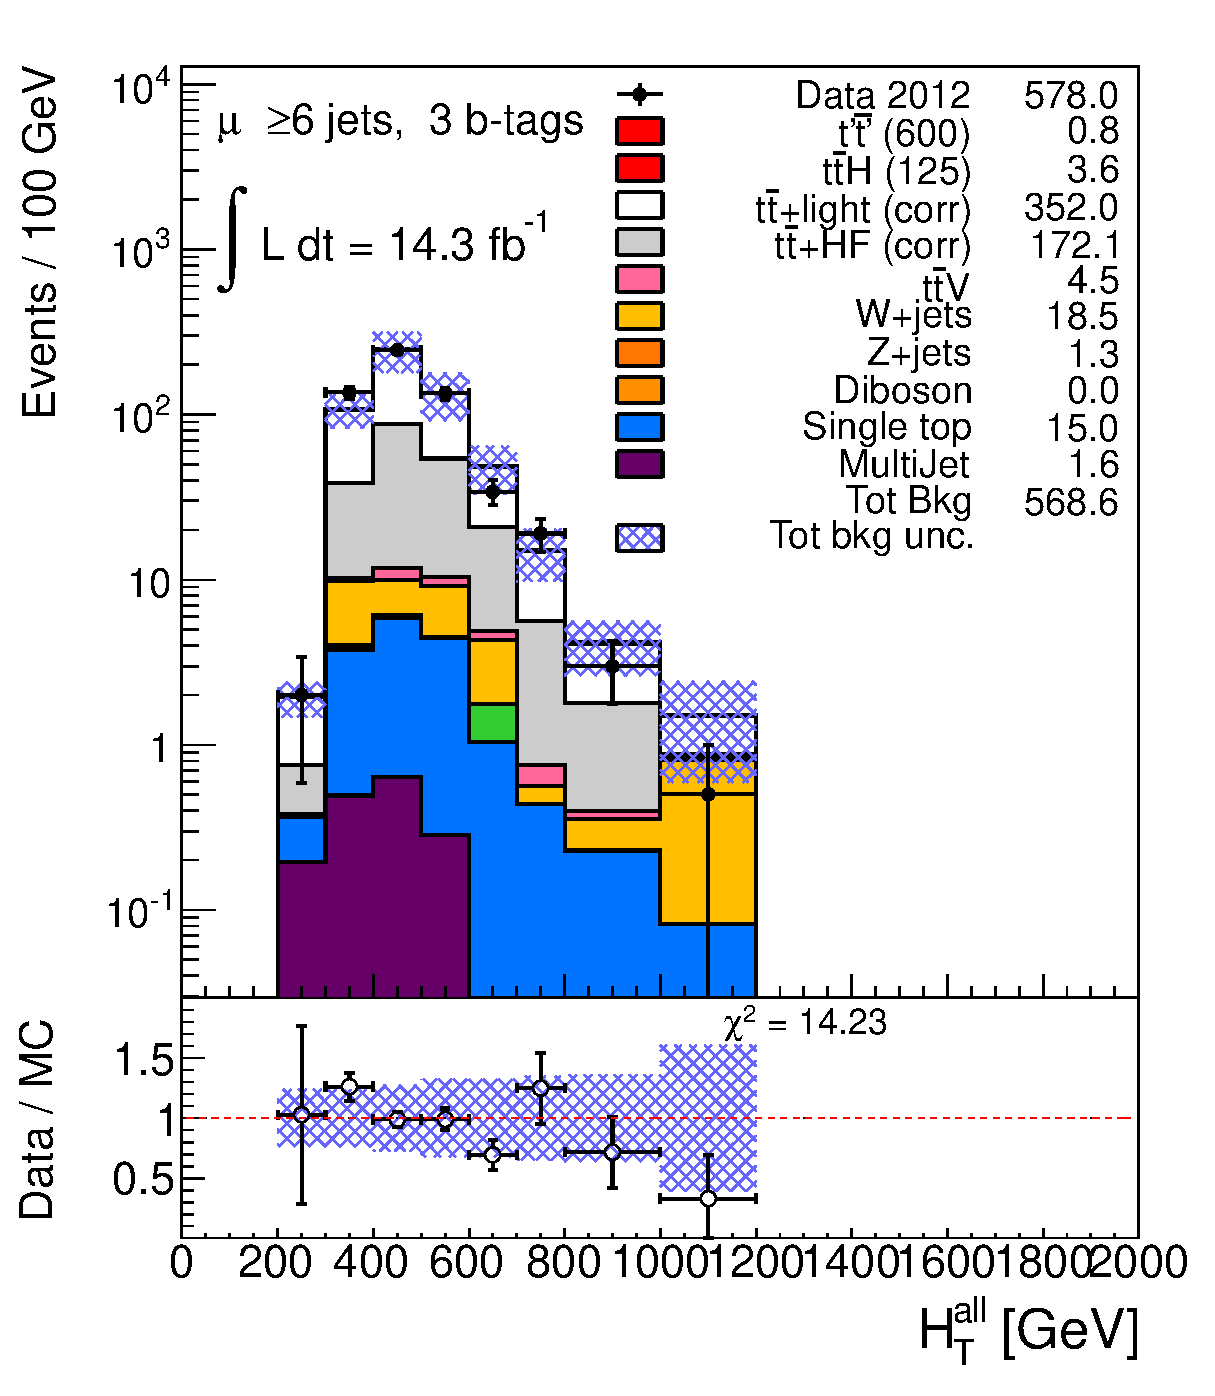
\includegraphics[width=0.3\textwidth]{appendices/figures/htx_httail/HTAll_MUON_6jetin3btagex_NOMINAL_logscale.eps}}
	\subfigure[]{
  	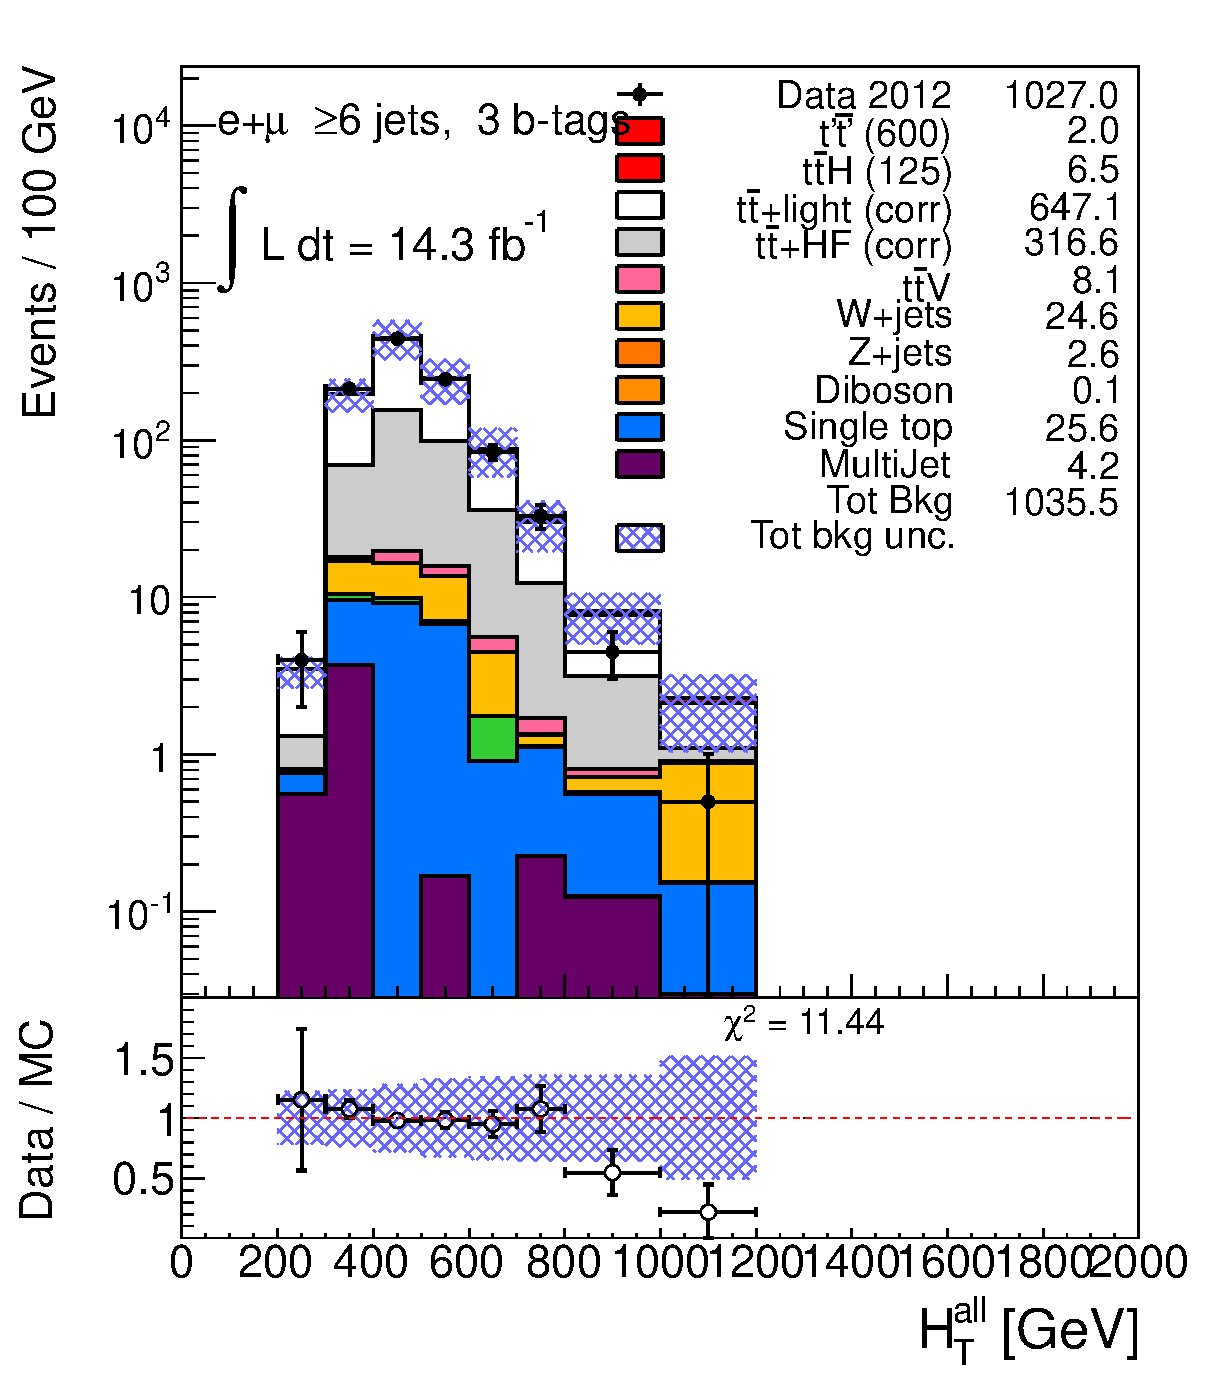
\includegraphics[width=0.3\textwidth]{appendices/figures/htx_httail/HTAll_ELEMUON_6jetin3btagex_NOMINAL_logscale.eps}}
	\caption{Data to Standard Model comparison for the $\HT$ variable in the $e$+jets, $\mu$+jets and combined channels,
        in the control regions specified in the text requiring 2 \btag ged jets (a--c) and 3 \btag ged jets (d--f).\label{fig:httailHTAll}}
\end{center}\end{figure}
